%\documentclass[handout]{beamer}
\documentclass[compress]{beamer}

%\documentclass{beamer}
\usepackage[T1]{fontenc}
\usepackage{pifont}
\usepackage{threeparttable}
\usepackage{subcaption}
\usepackage{tikz-qtree}
\usepackage{listings}
\usepackage[american]{babel}
\usepackage{csquotes}
\usepackage[style=apa, backend=biber]{biblatex}
\usepackage{tikz}
\usepackage{multicol}
\usepackage{booktabs}
\usepackage{graphicx}
\usepackage{neuralnetwork}
\usepackage{hyperref}

\usepackage{minted}
\definecolor{listingbg}{rgb}{0.87,0.93,1}
\setminted[python]{
breaklines,
linenos,
fontsize=\scriptsize,
frame=single,
xleftmargin=0pt}

\hypersetup{
    pdfborder={0 0 0},
    colorlinks=true,
}
\usetheme[block=fill,subsectionpage=progressbar,sectionpage=progressbar]{metropolis} 

\definecolor{Purple}{HTML}{911146}
\definecolor{Orange}{HTML}{CF4A30}

\setbeamercolor{alerted text}{fg=Orange}
\setbeamercolor{frametitle}{bg=Purple}

\setbeamercovered{still covered={\opaqueness<1->{5}},again covered={\opaqueness<1->{100}}}

\lstset{
    basicstyle=\scriptsize\ttfamily,
    columns=flexible,
    breaklines=true,
    numbers=left,
    %stepsize=1,
    numberstyle=\tiny,
    backgroundcolor=\color[rgb]{0.85,0.90,1}
}

\lstnewenvironment{lstlistingoutput}{\lstset{
        basicstyle=\footnotesize\ttfamily,
        columns=flexible,
        breaklines=true,
        numbers=left,
        %stepsize=1,
        numberstyle=\tiny,
        backgroundcolor=\color[rgb]{.7,.7,.7}}}{}


\lstnewenvironment{lstlistingoutputtiny}{\lstset{
        basicstyle=\tiny\ttfamily,
        columns=flexible,
        breaklines=true,
        numbers=left,
        %stepsize=1,
        numberstyle=\tiny,
        backgroundcolor=\color[rgb]{.7,.7,.7}}}{}

\renewcommand*{\bibfont}{\tiny}

\makeatletter
\setbeamertemplate{headline}{%
    \begin{beamercolorbox}[colsep=1.5pt]{upper separation line head}
    \end{beamercolorbox}
    \begin{beamercolorbox}{section in head/foot}
        \vskip2pt\insertnavigation{\paperwidth}\vskip2pt
    \end{beamercolorbox}%
    \begin{beamercolorbox}[colsep=1.5pt]{lower separation line head}
    \end{beamercolorbox}
}
\makeatother

\newcommand{\question}[1]{
    \begin{frame}[plain]
        \begin{columns}
            \column{.4\textwidth}
            \makebox[\columnwidth]{
                
\includegraphics[width=\columnwidth,height=\paperheight,keepaspectratio]{mannetje.png}}
            \column{.6\textwidth}
            \large
            \textcolor{orange}{\textbf{\emph{#1}}}
        \end{columns}
    \end{frame}}

\newcommand{\instruction}[1]{\emph{\textcolor{gray}{[#1]}}}

\addbibresource{../resources/literature.bib}
\graphicspath{{../resources/pictures/}}

\title[Computational Communication Science 2]{\textbf{Computational Communication Science 2} \\Week 6 - Lecture\\ »Validation (in Supervised Machine Learning)«}
\author[Marthe Möller]{a.m.moller@uva.nl}\author[A. Marthe Möller]{Marthe Möller \\ ~ \\ \footnotesize{a.m.moller@uva.nl} \\}
\date{May 6, 2024}
\institute[Digital Society Minor, University of Amsterdam]{Digital Society Minor, University of Amsterdam}


\begin{document}
	
	\begin{frame}{}
		\titlepage
	\end{frame}
	
	\begin{frame}{Today}
		\begin{tiny}
			\tableofcontents
		\end{tiny}
	\end{frame}


\section{Recap}

\begin{frame}[fragile]{Recap} 
	
\begin{alertblock}{Last week, we discussed:}
\begin{itemize}
	\item Supervised Machine Leaning (SML)
	\item The principles behind SML
	\item The steps of SML
	\item Some commonly used ML models
\end{itemize}
\end{alertblock}
	
\begin{alertblock}{At home, you:}
\begin{itemize}
	\item Got some hands-on experience SML (week 4 exercises)
\end{itemize}
\end{alertblock}	
\end{frame}


\begin{frame}[fragile]{Recap} 
\begin{alertblock}{Today, we:}
\begin{itemize}
	\item Review your first SML experience
	\item  Take a deep dive into validating SML-models
\end{itemize}
\end{alertblock}
	
\end{frame}


\begin{frame}[fragile]{Recap} 
	
\begin{alertblock}{Last week, you practiced with code that:}
\begin{itemize}
	\item Read in some data (Q1)
 	\item Split the data into a train and a test set (Q2)
	\item Set up a Count vectorizer (Q3)
	\item Trained a Naïve Bayes model with the count vectorizer (Q4)
	\item Requested some metrics for validation (Q5)
\end{itemize}
\end{alertblock}

\end{frame}


\begin{frame}[fragile]{Recap Q1}
	
\begin{lstlisting}
import csv
from collections import Counter
import matplotlib.pyplot as plt
			
file = "hatespeech_text_label_vote_RESTRICTED_100K.csv"
tweets = []
labels = []
		
with open(file) as fi:
  data = csv.reader(fi, delimiter='\t')
  for row in data:
   tweets.append(row[0])
   labels.append(row[1])
		
print(len(tweets) == len(labels)) # there should be just as many tweets as there are labels
		
Counter(labels)
plt.bar(Counter(labels).keys(), Counter(labels).values())
\end{lstlisting}

% you need two lists! 
\end{frame}



\begin{frame}[fragile]{Recap Q2}
Split the dataset:
\begin{lstlisting}
from sklearn.model_selection import train_test_split
		
tweets_train, tweets_test, y_train, y_test = train_test_split(tweets, labels, test_size=0.2, random_state=42)
\end{lstlisting}
	
%What is the random_state?
%What is test_size?
\end{frame}


\begin{frame}[fragile]{Recap Q3}
What happens here?
\begin{lstlisting}
from sklearn.feature_extraction.text import (CountVectorizer)
		
countvectorizer = CountVectorizer(stop_words="english")
X_train = countvectorizer.fit_transform(tweets_train)
X_test = countvectorizer.transform(tweets_test)
\end{lstlisting}
%Remember from the first lectures? Same technique for a different goal!
\end{frame}



\begin{frame}[fragile]{Recap Q4}
The actual SML part (yes, truly, it is three lines of code!):
\begin{lstlisting}
nb = MultinomialNB()
nb.fit(X_train, y_train)
y_pred = nb.predict(X_test)
\end{lstlisting}
%No output?
\end{frame}

\begin{frame}[fragile]{Recap Q5}
You can check what was created:
\begin{lstlisting}
nb = MultinomialNB()
nb.fit(X_train, y_train)
y_pred = nb.predict(X_test)

print(y_pred[:10])
\end{lstlisting}
	
\begin{lstlistingoutput}
['normal' 'normal' 'normal' 'normal' 'spam' 'normal' 'normal' 'normal' 'abusive' 'normal']
\end{lstlistingoutput}
\end{frame}


\begin{frame}[fragile]{Recap Q5}
Classification report:
\begin{lstlisting}
from sklearn.metrics import classification_report
		
print(classification_report(y_test, y_pred))
\end{lstlisting}
	
%Learn from the documentation!
\end{frame}


\begin{frame}{Up next}
	
Classification report: validate your classifier. \\\
	
More about this today!
\end{frame}


\section{Validating models}

\begin{frame}{Validation}
Validation: When we assess the "fit" between the theoretical concept that is studied and the obtained measures (Birkenmaier et al., 2023) \\\
\pause
Or when we try to answer the question: "How well does the classifier work?"
\end{frame}

\begin{frame}{Validation}
What criteria should we use to decide on this?\\\
\pause
Entirely context specific!
\end{frame}


\begin{frame}[fragile]{Validation}
\begin{alertblock}{Compare different goals for using SML:}
	\begin{itemize}
		\item To automatically decide what Instagram users should see an advertisement
		\item To automatically remove spam from Twitter feed
	\end{itemize}
\end{alertblock}

Would you use the same criterion in both cases to determine how well a classifier works? Why (not)?
\end{frame}


\begin{frame}[fragile]{Validation}
There are various evaluation metrics available for machine learning. \\\
In scikit-learn, they are presented by ways of a classification report!
\end{frame}


\begin{frame}[fragile]{Zooming out} 
	
\begin{alertblock}{So far, we:}
\begin{itemize}
	\item Reviewed the exercise and the basic steps of SML
	\item Talked about what validation is
\end{itemize}
\end{alertblock}
	
\begin{alertblock}{Next, we will talk about:}
\begin{itemize}
	\item Some commonly used validation metrics
	\item Input for SML
	\item Finding the best classifier
\end{itemize}
\end{alertblock}	
\end{frame}

\section{Validation metrics}

\begin{frame}[fragile]{Precision}
Precision quantifies the number of positive class predictions that actually belong to the positive cases. \\\ 
\pause
OR: How much of what we found is actually correct?
\end{frame}

\begin{frame}{Precision}
Precision quantifies the number of positive class predictions that actually belong to the positive cases. \\\ 
OR: How much of what we found is actually correct? \\\


\begin{alertblock}{Compare different goals for using SML:}
\begin{itemize}
	\item To automatically decide what Instagram users should see an advertisement
	\item To automatically remove spam from Twitter feed
\end{itemize}
\end{alertblock}
\end{frame}



\begin{frame}{Recall}
Recall quantifies the number of positive class prediction made out of all positive examples in the dataset. \\\
\pause
OR: How many of the cases that we wanted to find did we actually find?
\end{frame}


\begin{frame}{Recall}
Recall quantifies the number of positive class prediction made out of all positive examples in the dataset. \\\
OR: How many of the cases that we wanted to find did we actually find?
	
\begin{alertblock}{Compare different goals for using SML:}
\begin{itemize}
	\item To automatically decide what Instagram users should see an advertisement
	\item To automatically remove spam from Twitter feed
\end{itemize}
\end{alertblock}
\end{frame}

\begin{frame}{Precision and Recall}
\begin{center}
	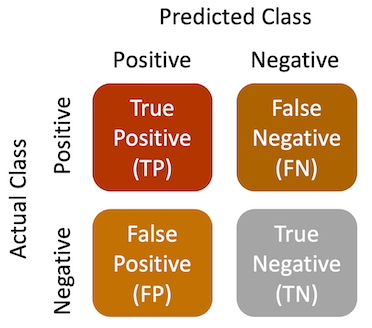
\includegraphics[width=\linewidth,height=\textheight,keepaspectratio]{../pictures/confusionmatrix_words.png} \\\
\end{center}
\end{frame}

\begin{frame}{Precision and Recall} 
	
\begin{columns}
	\column{.3\textwidth}
	\makebox[\columnwidth]{
		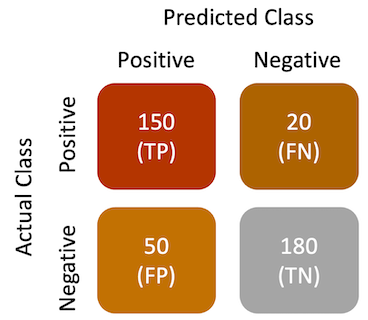
\includegraphics[width=\columnwidth,height=\paperheight,keepaspectratio]{../pictures/confusionmatrix_numbers.png}}
	\column{.7\textwidth}
	Precision is calculated as: \(\frac{\rm{TP}}{\rm{TP}+\rm{FP}}\) \\\
	In this example \(\frac{\rm{150}}{\rm{150}+\rm{50}}\) which is \(0.75\) \\\
	Recall is calculated as \(\frac{\rm{TP}}{\rm{TP}+\rm{FN}}\) \\\
	In this example \(\frac{\rm{150}}{\rm{150}+\rm{20}}\) which is \(0.88\)
\end{columns}
\end{frame}


\begin{frame}[fragile]{What does this look like in code?}
	
Let's ask for a confusion matrix: 
\begin{lstlisting}
from sklearn.metrics import confusion_matrix
		
y_test = [0, 1, 1, 1, 0]
y_pred = [0, 0, 1, 1, 1]
		
print(confusion_matrix(y_test, y_pred))
\end{lstlisting}
	
\begin{lstlistingoutput}
[[1  1 ]
[ 1  2]]
\end{lstlistingoutput}
\end{frame}

\begin{frame}[fragile]{The classification report}
	
Let's get some metrics for validation: 
	
\begin{lstlisting}
from sklearn.metrics import classification_report
print(classification_report(y_test, y_pred))
\end{lstlisting}

\begin{center}
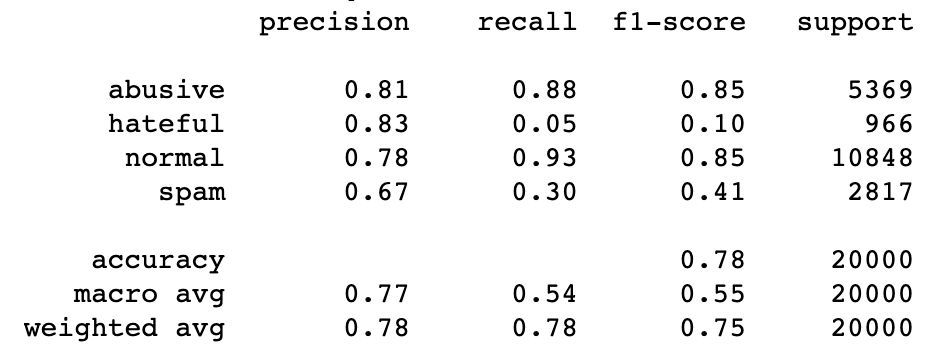
\includegraphics[width=\linewidth,height=\textheight,keepaspectratio]{../pictures/classification-report} \\\
\end{center}

\end{frame}


\begin{frame}{\(F_1\)-score}
But wait...

\begin{alertblock}{Compare different goals for using SML:}
\begin{itemize}
	\item To automatically decide what Instagram users should see an advertisement
	\item To automatically remove spam from Twitter feed
\end{itemize}
\end{alertblock}

Such information was not available in the exercise for last week!

%How do you know what is best - precision or recall?
\end{frame}


\begin{frame}{\(F_1\)-score}
\(F_1\)-score: The harmonic mean of precision and recall.
(Weighted average of precision and recall) \\
	
\(F_1\)-score \(= 2 \cdot \frac{\rm precision \cdot recall}{\rm precision + recall}\)
\end{frame}


\begin{frame}[fragile]{Accuracy}
	
\begin{center}
	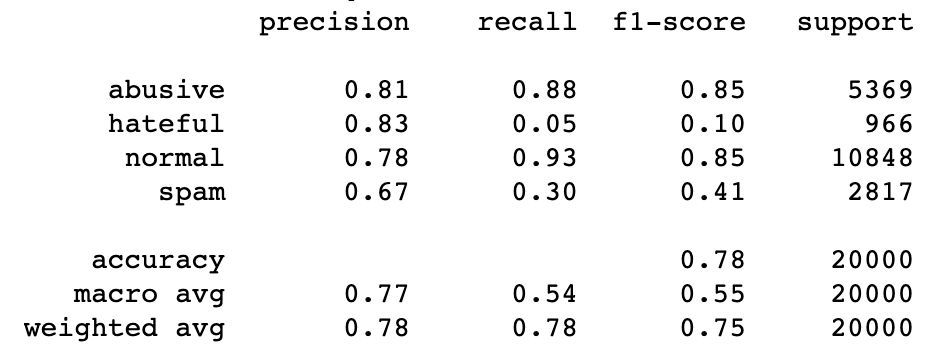
\includegraphics[width=\linewidth,height=\textheight,keepaspectratio]{../pictures/classification-report} \\\
\end{center}
	
\end{frame}

\begin{frame}{Accuracy}
Accuracy: In which percentage of all cases was our classifier right? \\

% Rather general, always useful?
\end{frame}


\begin{frame}{Accuracy}
	
Class distribution: The number of examples that belong to each class. \\
	
Imbalanced classification: A predictive modeling problem where the distribution of examples across the classes within a training dataset is not equal.
	
% Not useful if you are dealing with class imbalance!
\end{frame}


\begin{frame}[fragile]{Accuracy}
\begin{center}
	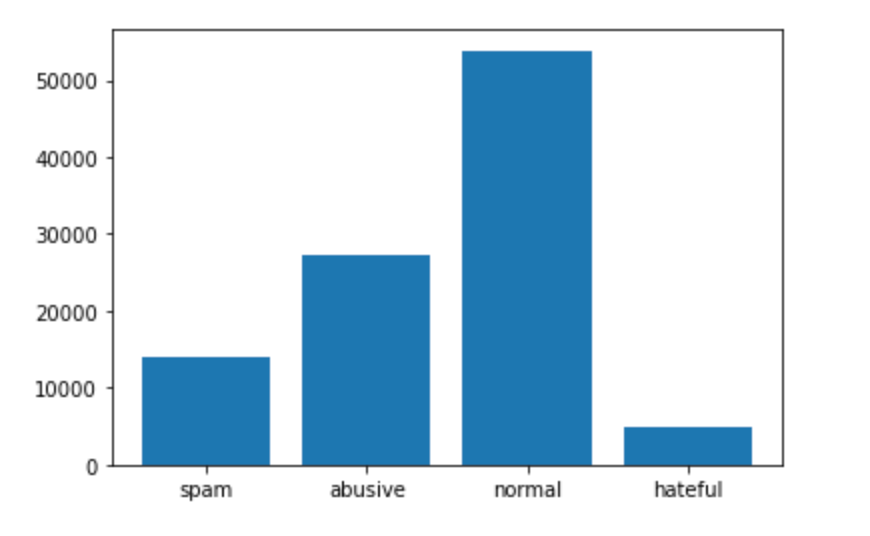
\includegraphics[width=\linewidth,height=\textheight,keepaspectratio]{../pictures/barplot} \\\
\end{center}
\end{frame}

\begin{frame}{Accuracy}
	
\begin{center}
	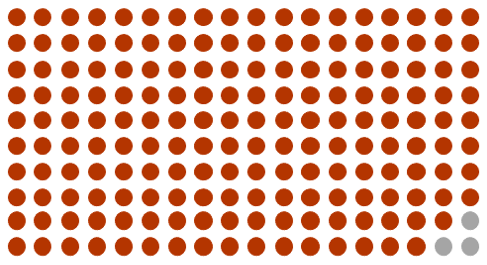
\includegraphics[width=\linewidth,height=\textheight,keepaspectratio]{../pictures/imbalance.png} 
\end{center}	

Majority class (red dots) vs. minority class (grey dots) 
\end{frame}

\begin{frame}{Accuracy}
Always check how your cases are distributed across the labels. \\
If your training data overrepresents certain cases, be aware of its potential consequences.\\
More about the consequences of bad input data next week!
\end{frame}

\begin{frame}{Validation: Best practices}
Back to this question: \\
How do you know what metric is most suitable to assess your model?
\end{frame}


\begin{frame}{Validation: Best practices}
Decide what metric is best to use beforehand.

\begin{alertblock}{Consider:}
	\begin{itemize}
		\item What does a specific metric tell you? How does this relate to your question?
		\item Is class imbalance an issue? 
		\item What will the classifier be used for? How much room is there for errors?
	\end{itemize}
\end{alertblock}

The latter can bring you back to the question: To SML or not to SML?
\end{frame}

\begin{frame}{Validation: Best practices}

\begin{alertblock}{SML suitability depends on:}
\begin{itemize}
	\item How hard/easy it is to translate the decision proces for classification into straight-forward rules
	\item How much data there are to classify
	\item How much room there is for errors 
\end{itemize}
\end{alertblock}
\end{frame}

\begin{frame}[fragile]{Zooming out} 
	
	\begin{alertblock}{So far, we:}
		\begin{itemize}
			\item Reviewed the exercise and the basic steps of SML
			\item Talked about what validation is
			\item Discussed some commonly used validation metrics
		\end{itemize}
	\end{alertblock}

	\begin{alertblock}{Next, we will talk about:}
		\begin{itemize}
			\item Additional validation methods
		\end{itemize}
	\end{alertblock}	
\end{frame}


\section{Additional validation methods}

\begin{frame}{Birkenmaier et al., 2023}
Comparison to human-annotations is one way to assess (external) validity. \\
More options are available, although used less frequently.
\end{frame}

\begin{frame}{Birkenmaier et al., 2023}
\begin{alertblock}{Additional approaches:}
	\begin{itemize}
		\item Justification of pre-processing steps
		\item Inspecting descriptive statistics
		\item Qualitative (error) analysis
		\item Report on the rejection of poorly performing models
	\end{itemize}
\end{alertblock}

Yet, validation remains hard for scholars working with CTAM. Why?
\end{frame}

% Becuse there is no clear consensus on how researchers should validate their text-based measures.

\begin{frame}{Birkenmaier et al., 2023}
	\begin{alertblock}{Recommendations}
		\begin{itemize}
			\item Justify concstructs and outline operationalizations
			\item Always validate CTAM
			\item Combine internet and external validation
			\item Always compare to human annotations
			\item Maximize transparency and reproducibility 
		\end{itemize}
	\end{alertblock}
\end{frame}


\begin{frame}{Validation: Best practices}
In last week's lecture, we saw that you can train many different classifiers.  

\begin{alertblock}{Amongst other, classifiers can differ based on:}
	\begin{itemize}
		\item The vectorizer that is used on the data (i.e., count vectorizer or tf-idf vectorizer)
		\item The underlying model (e.g., Naïve Bayes, Logistic Regression, Decision Trees, SVM, etc.)\\\
	\end{itemize}
\end{alertblock}
\pause
Knowing about validation methods, you may wonder:
How do you know what classifier is best beforehand?
\end{frame}


\begin{frame}{Selecting a classifier}

You don't!\\\
\pause
Typically, various classifiers are trained and their performance is compared.\\\
\pause
The best performing classifier is then selected and used to annotate more/new data.
%iterative process
\end{frame}


\begin{frame}{Selecting a classifier}
Heed Birkenmaier atl.'s (2023) advice and explicitely discuss and argue for your choices.
\end{frame}


\begin{frame}[fragile]{Zooming out} 
	
\begin{alertblock}{Today, we:}
\begin{itemize}
	\item Reviewed the exercise and the basic steps of SML
	\item Talked about what validation is
	\item Discussed some commonly used validation metrics
	\item Looked beyond the commonly used validation metrics
\end{itemize}
\end{alertblock}
	
\end{frame}


\begin{frame}[fragile]{Zooming out} 
	
\begin{alertblock}{Tomorrow and this week, you will:}
\begin{itemize}
	\item Set up multiple different classifiers
	\item Validate those classifiers
	\item Select the best performing classifier
\end{itemize}
\end{alertblock}
	
Work on the tutorial exercises for this week. \\\
\end{frame}


\end{document}